%% PeerJ Computer Science submission
%% Compiled with: pdflatex main.tex / bibtex main / pdflatex main.tex / pdflatex main.tex
%% Line-numbering enabled for peer-review submission (remove 'lineno' for camera-ready)

\documentclass[fleqn,10pt,lineno]{wlpeerj}

%% -----------------------------------------------
%% Additional packages (not pre-loaded by wlpeerj)
%% -----------------------------------------------
\usepackage{amsmath,amssymb}
\usepackage{booktabs}
\usepackage{tabularx}
\usepackage{float}
\usepackage{enumitem}

%% Custom column types for tabularx
\newcolumntype{C}{>{\centering\arraybackslash}X}
\newcolumntype{L}{>{\raggedright\arraybackslash}X}

%% -----------------------------------------------
%% Article Metadata
%% -----------------------------------------------
\title{AI-based prediction and monitoring system for acute myocardial infarction detection using laboratory biomarkers: a comparative machine learning study with temporal feature engineering}

\author[1]{Hussam Aziz Ayed Alshammari}
\author[1]{Abdullah Eyada Mutlaq Alshammari}

\affil[1]{Artificial Intelligence and Data Science Department,
          College of Computer Science and Engineering,
          University of Hail, Hail 2440, Saudi Arabia}

\corrauthor[1]{Hussam Aziz Ayed Alshammari}{Husam.a.ayed@gmail.com}

% Keywords are declared inside the document body for this wlpeerj.cls version

%% -----------------------------------------------
%% Abstract (must appear before \begin{document})
%% -----------------------------------------------
\begin{abstract}
Early and accurate detection of myocardial infarction (MI) is critical for timely clinical intervention and improved patient outcomes. This study presents an AI-based prediction and monitoring system for acute MI detection using laboratory biomarkers, specifically troponin and creatine kinase-MB (CK-MB). The proposed system is designed to support clinical decision-making by providing automated risk stratification and continuous patient monitoring across multiple hospital visits. A rigorous nested cross-validation methodology with patient-level stratification is employed to ensure unbiased performance estimation and prevent data leakage. This study compares four machine learning classifiers---Logistic Regression, Random Forest, Histogram Gradient Boosting (HGB), and XGBoost---on a clinical dataset comprising 2,327 hospital visits from 1,506 unique patients. Temporal feature engineering techniques, including delta changes between consecutive biomarker measurements, maximum prior values, and visit-level tracking, enable continuous patient monitoring. The XGBoost classifier achieved the highest performance with a precision-recall area under curve (PR-AUC) of 0.986 and a receiver operating characteristic area under curve (ROC-AUC) of 0.982, while maintaining a clinically mandated target recall of 98\%. Ensemble methods (XGBoost, HGB, Random Forest) substantially outperformed Logistic Regression, achieving F1-scores exceeding 0.94 compared to 0.87. The results demonstrate that modern gradient boosting methods can serve as effective clinical decision support tools for MI detection, with particular strength in exploiting temporal biomarker dynamics for continuous patient monitoring applications.
\end{abstract}

\begin{document}

\flushbottom
\maketitle
\thispagestyle{empty}

\noindent\textbf{Keywords:} Myocardial infarction; machine learning; XGBoost; cardiac biomarkers; clinical decision support; temporal feature engineering; nested cross-validation; troponin; CK-MB; random forest


%%=========================================================
\section*{Introduction}
%%=========================================================

Myocardial infarction (MI), commonly known as heart attack, remains one of the leading causes of mortality worldwide~\citep{Thygesen2018}. Early detection and timely intervention are crucial factors in reducing MI-related morbidity and mortality. The diagnosis of MI traditionally relies on clinical symptoms, electrocardiogram (ECG) findings, and elevated cardiac biomarkers, particularly cardiac troponin~\citep{Amsterdam2014, Collet2021}.

Cardiac troponin has become the gold standard biomarker for MI diagnosis due to its high sensitivity and specificity for myocardial injury~\citep{Reichlin2009, Chapman2020}. Creatine kinase-MB (CK-MB), while less specific than troponin, continues to serve as a valuable complementary marker in clinical practice~\citep{Aydin2019}. The interpretation of these biomarkers, however, can be challenging due to their time-dependent release kinetics and the need to consider serial measurements.

In emergency department settings, clinicians face the critical challenge of making rapid diagnostic decisions under time pressure and high patient volumes. The accurate interpretation of laboratory biomarker patterns, particularly when monitoring patients across multiple visits, requires integration of complex temporal information that can exceed human cognitive capacity. Artificial intelligence (AI) systems offer a promising solution to augment clinical decision-making by automatically analyzing biomarker trajectories, identifying high-risk patterns, and providing real-time risk stratification to support physician judgment.

Machine learning (ML) approaches have shown promise in various medical diagnostic applications, including cardiovascular disease prediction~\citep{Attia2019, Rajkomar2019, Topol2019}. These methods can capture complex non-linear relationships between multiple variables and potentially improve diagnostic accuracy beyond traditional rule-based approaches. When integrated into clinical workflows, AI-based decision support tools can reduce diagnostic delays, minimize missed diagnoses, and enable more efficient allocation of healthcare resources~\citep{Wiens2019}.

Despite the growing interest in ML-based MI detection, several methodological challenges remain. Many existing studies suffer from data leakage due to improper cross-validation strategies that do not account for patient-level dependencies~\citep{Varoquaux2022}. Additionally, comparative studies of multiple ML algorithms on the same dataset with consistent evaluation methodology are relatively scarce.

This study addresses these gaps by presenting a rigorous comparative analysis of four ML algorithms---Logistic Regression, Random Forest, HGB, and XGBoost---for MI detection using cardiac biomarkers. A nested cross-validation framework with patient-level stratification is employed to ensure unbiased model selection and performance estimation. The primary objective is to identify the most effective ML approach for MI detection while maintaining a clinically relevant target recall of 98\%.

The main contributions of this work are:
\begin{enumerate}[noitemsep]
\item A comprehensive comparison of four ML algorithms for MI detection using a rigorous nested cross-validation methodology.
\item Implementation of patient-level stratification to prevent data leakage and ensure generalizable performance estimates.
\item Development of temporal feature engineering techniques that capture the dynamic nature of biomarker changes across multiple hospital visits.
\item Threshold optimization to achieve a target recall of 98\%, suitable for clinical screening applications.
\item A clinical decision support framework designed to enhance healthcare delivery through automated risk stratification and continuous patient monitoring.
\end{enumerate}

The proposed AI-based system has the potential to significantly enrich the healthcare sector by addressing several critical challenges: reducing diagnostic delays that can lead to increased mortality, providing 24/7 automated screening capability in understaffed facilities, enabling objective and consistent interpretation of complex biomarker patterns, and supporting evidence-based clinical decision-making in high-pressure emergency settings.

%%=========================================================
\section*{Related Work}
%%=========================================================

Machine learning applications in cardiovascular disease detection have grown substantially in recent years. \citet{Topol2019} provided a comprehensive overview of how AI is transforming clinical medicine, while \citet{Attia2019} demonstrated the potential of deep learning for detecting various cardiac conditions from ECG signals, achieving remarkable accuracy in identifying previously undiagnosed conditions. Deep neural networks applied to ECG data have also shown promise for mortality prediction~\citep{Raghunath2020}.

In the context of biomarker-based MI detection, several studies have explored ML approaches. \citet{Than2019} developed decision support tools combining clinical features with troponin values to improve risk stratification in patients with suspected acute coronary syndrome. Their work highlighted the importance of serial biomarker measurements in improving diagnostic accuracy. The kinetics of high-sensitivity cardiac troponin, including the characteristic rise-and-fall pattern, have been extensively studied as the cornerstone of MI diagnosis under the Fourth Universal Definition~\citep{Chapman2020, Collet2021}. \citet{Body2021} demonstrated that undetectable troponin levels at presentation could be used for rapid rule-out of MI using high-sensitivity assays, further establishing the value of biomarker-based decision pathways.

A recent systematic review by \citet{Alahmadi2024} surveyed ML approaches for heart disease prediction, identifying troponin levels and ensemble methods as key components in achieving high diagnostic accuracy. The review emphasized the need for rigorous evaluation methodologies and external validation to ensure clinical applicability.

Ensemble methods have shown particular promise in medical diagnosis. Gradient boosting algorithms, including XGBoost~\citep{Chen2016} and LightGBM~\citep{Ke2017}, have demonstrated superior performance in various healthcare prediction tasks. Random Forest~\citep{Breiman2001}, one of the earliest ensemble learning methods, continues to serve as a robust baseline in clinical studies. These methods effectively handle heterogeneous data types and can capture complex feature interactions.

The importance of proper evaluation methodology in medical ML has been emphasized by several authors. \citet{Varoquaux2022} highlighted common pitfalls in ML studies, including inappropriate cross-validation strategies that lead to over-optimistic performance estimates. Nested cross-validation has been recommended as the gold standard for unbiased model selection and evaluation~\citep{Cawley2010}. The choice of evaluation metrics is equally critical: \citet{Saito2015} demonstrated that precision-recall curves are more informative than ROC curves for imbalanced datasets, while \citet{Hicks2022} provided comprehensive recommendations for evaluation metrics in medical AI applications. Furthermore, \citet{Obermeyer2019} highlighted the risk of algorithmic bias in healthcare applications, underscoring the importance of fairness-aware model development.

The responsible deployment of ML in clinical settings requires careful consideration of potential harms. \citet{Wiens2019} outlined a roadmap for responsible ML in healthcare, advocating for transparency, interpretability, and rigorous validation. Explainability methods such as SHAP values~\citep{Lundberg2020} have become essential tools for understanding model predictions and building clinician trust in AI-based decision support systems.

%%=========================================================
\section*{Materials and Methods}
%%=========================================================

Figure~\ref{fig:workflow} presents an overview of the complete methodology employed in this study, from data collection through model evaluation.

\begin{figure}[htbp]
\centering
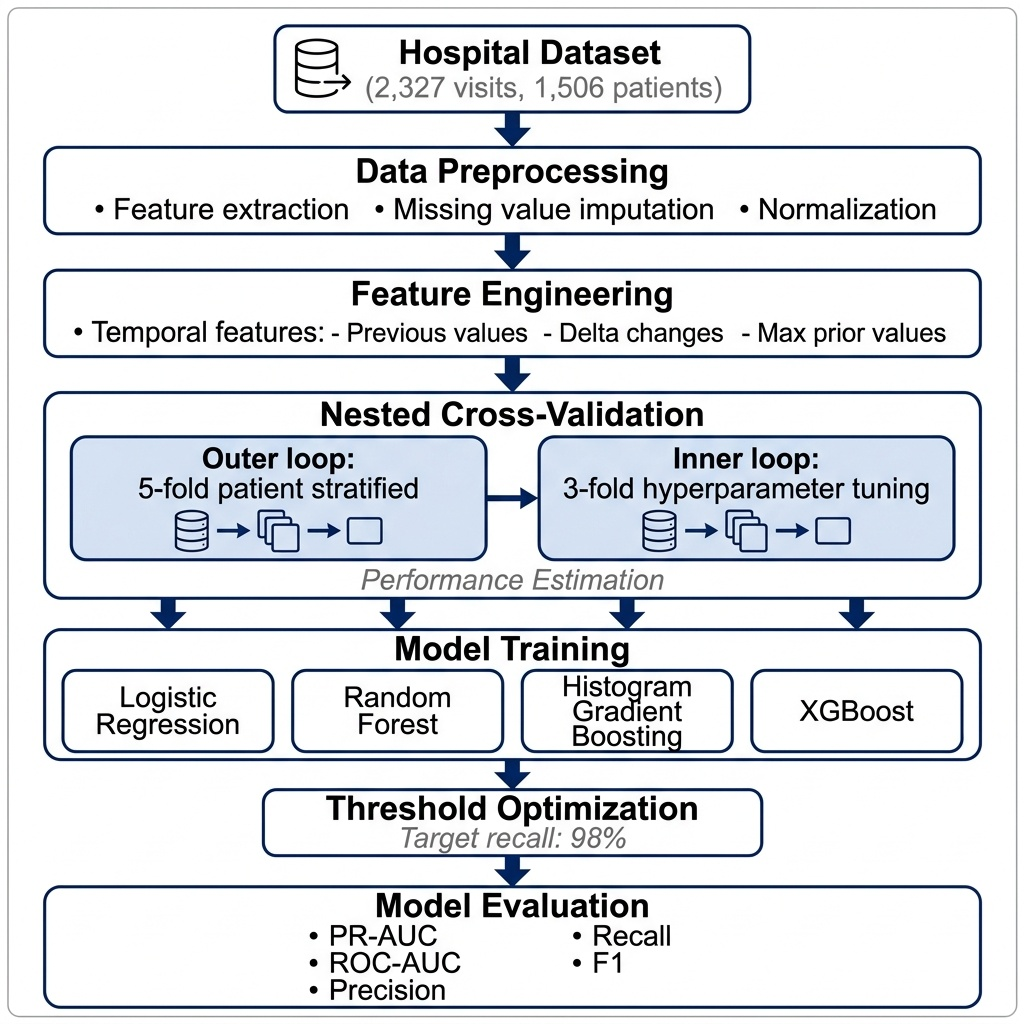
\includegraphics[width=\textwidth, keepaspectratio]{fig_workflow_hires.jpeg}
\caption{Workflow diagram of the proposed MI detection methodology. The pipeline includes data preprocessing, temporal feature engineering, nested cross-validation with patient-level stratification, training of four ML classifiers, threshold optimization for 98\% recall, and comprehensive model evaluation.}
\label{fig:workflow}
\end{figure}

\subsection*{Dataset Description}

The study utilized a hospital diagnosis dataset containing 2,327 patient visits from 1,506 unique patients. Each record included clinical and laboratory measurements obtained during hospital visits. The dataset was de-identified by replacing patient identifiers with cryptographic hashes to protect patient privacy.

The target variable was defined as acute MI based on ICD-10 codes I21 (ST-elevation and non-ST-elevation myocardial infarction) and I22 (subsequent myocardial infarction), as well as keyword matching in diagnosis text including ``myocardial infarction,'' ``STEMI,'' and ``NSTEMI.'' Cases containing terms such as ``history of'' or ``old MI'' were excluded to focus on acute events. The dataset exhibited a positive rate of 57.5\% at the visit level, with 647 positive patients and 859 negative patients.

\subsection*{Feature Engineering}

The raw dataset was processed to extract clinically meaningful features. Numerical features included patient age, troponin levels, and CK-MB values. Categorical features included visit type. All numerical features underwent median imputation for missing values followed by standardization using z-score normalization.

To capture the temporal dynamics of biomarker changes, which are clinically important for MI diagnosis, several derived features were engineered:
\begin{itemize}[noitemsep]
\item \textbf{Previous values}: The immediately preceding troponin and CK-MB measurements for each patient.
\item \textbf{Delta changes}: The difference between current and previous biomarker values.
\item \textbf{Maximum prior}: The maximum observed biomarker value up to the previous visit.
\item \textbf{Visit index}: A sequential counter of visits for each patient.
\item \textbf{Days since last visit}: The temporal gap between consecutive visits.
\end{itemize}

Table~\ref{tab:features} presents the complete feature inventory used in this study.

\begin{table}[ht]
\small
\begin{tabularx}{\linewidth}{llL}
\toprule
\textbf{Feature} & \textbf{Type} & \textbf{Description} \\
\midrule
age & Numerical & Patient age, standardized \\
visit\_type & Categorical & Visit context (one-hot encoded) \\
visit\_index & Numerical & Sequential visit counter per patient \\
days\_since\_last\_visit & Numerical & Days between consecutive visits \\
troponin & Numerical & Current troponin level \\
troponin\_prev & Numerical & Previous troponin measurement \\
troponin\_delta & Numerical & Change from previous troponin \\
troponin\_max\_prior & Numerical & Maximum prior troponin value \\
ckmb & Numerical & Current CK-MB level \\
ckmb\_prev & Numerical & Previous CK-MB measurement \\
ckmb\_delta & Numerical & Change from previous CK-MB \\
ckmb\_max\_prior & Numerical & Maximum prior CK-MB value \\
\bottomrule
\end{tabularx}
\caption{Complete feature inventory for the MI prediction model.}
\label{tab:features}
\end{table}

This resulted in a total of 12 features: 11 numerical features and 1 categorical feature (visit type), which was one-hot encoded.

\subsection*{Machine Learning Models}

Four ML classifiers were evaluated in this study:

\paragraph{Logistic Regression}
A linear classifier with L2 regularization. The regularization strength parameter $C$ was tuned from $10^{-3}$ to $10^2$ on a logarithmic scale. Class weights were balanced to account for class imbalance.

\paragraph{Random Forest}
An ensemble of 600 decision trees with bootstrap aggregation. Tuned hyperparameters included maximum tree depth (3, 5, 8, or unlimited), minimum samples per leaf (1, 5, 10, 30), and maximum features (square root, log2, or all). Balanced subsample class weighting was applied.

\paragraph{Histogram Gradient Boosting (HGB)}
A gradient boosting implementation optimized for large datasets using histogram-based splitting. Tuned hyperparameters included maximum depth (3, 4, 5, unlimited), learning rate (0.02--0.1), maximum leaf nodes (15--127), minimum samples per leaf (10--80), and L2 regularization (0, 0.1, 1.0).

\paragraph{XGBoost}
An optimized gradient boosting implementation with 900 estimators. Tuned hyperparameters included maximum depth (3--6), learning rate (0.02--0.08), subsample ratio (0.7--1.0), column subsample ratio (0.7--1.0), and minimum child weight (1, 3, 5).

\subsection*{Algorithm Formulations}

\paragraph{Logistic Regression}
Logistic Regression models the probability of MI as a function of input features using the sigmoid function:
\begin{equation}
P(y=1|\mathbf{x}) = \sigma(\mathbf{w}^T\mathbf{x} + b) = \frac{1}{1 + e^{-(\mathbf{w}^T\mathbf{x} + b)}}
\label{eq:logreg}
\end{equation}
where $\mathbf{w}$ represents the weight vector, $\mathbf{x}$ is the feature vector, and $b$ is the bias term. With L2 regularization, the objective function becomes:
\begin{equation}
\min_{\mathbf{w},b} \sum_{i=1}^{n} \mathcal{L}(y_i, \hat{y}_i) + \frac{1}{C}\|\mathbf{w}\|_2^2
\label{eq:logreg_obj}
\end{equation}
where $C$ is the regularization strength parameter and $\mathcal{L}$ is the cross-entropy loss.

\paragraph{Random Forest}
Random Forest constructs an ensemble of $B$ decision trees and combines their predictions through averaging:
\begin{equation}
\hat{y} = \frac{1}{B}\sum_{b=1}^{B} f_b(\mathbf{x})
\label{eq:rf}
\end{equation}
where $f_b(\mathbf{x})$ represents the prediction of the $b$-th tree. In this study, $B=600$ trees were used with bootstrap aggregation to reduce variance and prevent overfitting.

\paragraph{Gradient Boosting (HGB and XGBoost)}
Gradient boosting methods build an additive model by iteratively fitting new trees to the residuals:
\begin{equation}
\hat{y}^{(t)} = \hat{y}^{(t-1)} + \eta \cdot f_t(\mathbf{x})
\label{eq:gb}
\end{equation}
where $\eta$ is the learning rate and $f_t$ is the tree added at iteration $t$. XGBoost minimizes the following regularized objective:
\begin{equation}
\mathcal{L}^{(t)} = \sum_{i=1}^{n} l(y_i, \hat{y}_i^{(t-1)} + f_t(\mathbf{x}_i)) + \Omega(f_t)
\label{eq:xgb_obj}
\end{equation}
where the regularization term is defined as:
\begin{equation}
\Omega(f) = \gamma T + \frac{1}{2}\lambda\sum_{j=1}^{T}w_j^2
\label{eq:xgb_reg}
\end{equation}
with $T$ being the number of leaves, $w_j$ the leaf weights, and $\gamma$, $\lambda$ the regularization parameters.

\paragraph{Evaluation Metrics}
Model performance was evaluated using the following metrics. Precision and recall are defined as:
\begin{equation}
\text{Precision} = \frac{TP}{TP + FP}, \quad \text{Recall} = \frac{TP}{TP + FN}
\label{eq:prec_rec}
\end{equation}
The F1-score provides the harmonic mean of precision and recall:
\begin{equation}
\text{F1} = 2 \cdot \frac{\text{Precision} \cdot \text{Recall}}{\text{Precision} + \text{Recall}}
\label{eq:f1}
\end{equation}
The area under the precision-recall curve (PR-AUC) and receiver operating characteristic curve (ROC-AUC) provide threshold-independent performance measures:
\begin{align}
\text{PR-AUC} &= \int_0^1 P(R) \, dR \label{eq:prauc} \\
\text{ROC-AUC} &= \int_0^1 TPR(FPR) \, d(FPR) \label{eq:rocauc}
\end{align}

\subsection*{Software Environment}

All experiments were implemented in Python 3.12.12, running on Google Colab. Key library versions were: scikit-learn 1.6.1, xgboost $\geq$1.7.0 (installed via \texttt{pip install xgboost}), pandas $\geq$2.0.0, numpy $\geq$1.24.0, and matplotlib $\geq$3.7.0. All stochastic operations were seeded with the fixed value \texttt{SEED = 42} to ensure full reproducibility.

\subsection*{Evaluation Methodology}

A nested cross-validation framework was employed to obtain unbiased performance estimates while performing hyperparameter optimization~\citep{Cawley2010}. The outer loop consisted of 5-fold stratified cross-validation with patient-level grouping, ensuring that all visits from a given patient appeared in either the training or test set, but not both. The inner loop used 3-fold stratified cross-validation for hyperparameter tuning via randomized search with 12 iterations.

For each outer fold, the best hyperparameters were selected based on average precision score (equivalent to PR-AUC) in the inner validation. The final model was trained on the entire outer training set and evaluated on the held-out test set.

Decision thresholds were optimized to achieve a target recall of 98\%, reflecting the clinical priority of minimizing missed MI diagnoses. For each fold, the threshold achieving at least 98\% recall with the highest precision was selected from the precision-recall curve computed on inner fold validation predictions.

Performance metrics included PR-AUC, ROC-AUC, precision, recall, and F1-score, all computed at the optimized threshold.

\subsection*{Hyperparameter Search Space}

Table~\ref{tab:hyperparams} summarizes the hyperparameter search spaces explored during nested cross-validation. Model selection was performed using RandomizedSearchCV with 12 iterations per fold, optimizing for average precision score.

\begin{table}[ht]
\small
\begin{tabularx}{\linewidth}{lL}
\toprule
\textbf{Model} & \textbf{Hyperparameter Search Space} \\
\midrule
LogReg & $C$: $10^{-3}$ to $10^{2}$ (12 log-spaced values) \\
\addlinespace
RF & max\_depth: \{3, 5, 8, None\}; min\_samples\_leaf: \{1, 5, 10, 30\}; max\_features: \{sqrt, log2, None\} \\
\addlinespace
HGB & max\_depth: \{3, 4, 5, None\}; learning\_rate: \{0.02, 0.03, 0.05, 0.08, 0.1\}; max\_leaf\_nodes: \{15, 31, 63, 127\}; min\_samples\_leaf: \{10, 20, 40, 80\}; L2\_regularization: \{0, 0.1, 1.0\} \\
\addlinespace
XGBoost & max\_depth: \{3, 4, 5, 6\}; learning\_rate: \{0.02, 0.03, 0.05, 0.08\}; subsample: \{0.7, 0.85, 1.0\}; colsample\_bytree: \{0.7, 0.85, 1.0\}; min\_child\_weight: \{1, 3, 5\} \\
\bottomrule
\end{tabularx}
\caption{Hyperparameter search spaces for each classifier.}
\label{tab:hyperparams}
\end{table}

The XGBoost classifier was initialized with 900 estimators and the histogram tree method for computational efficiency. Random Forest used 600 estimators with balanced subsample class weighting. All random operations were seeded with the fixed value 42 (\texttt{SEED = 42}) to ensure reproducibility, consistent with the nested cross-validation structure (outer: 5-fold, inner: 3-fold) confirmed in the experimental implementation. The target recall of 98\% was achieved by optimizing the classification threshold on the precision-recall curve from validation predictions.

\subsection*{Ethical Approval and Informed Consent}

This study was approved by the Institutional Review Board (IRB) of the Hail Health Cluster, Research and Studies Department, Hail Region, Kingdom of Saudi Arabia (IRB Log Number: 2025-13; Category: Expedited; Date of Approval: February 24, 2025). The approval was granted for the study entitled ``Cardiac Arrest Prediction and Monitoring Using Artificial Intelligence''. The study is retrospective in nature, utilizing a fully de-identified clinical dataset in which all direct and indirect patient identifiers were replaced with cryptographic hashes prior to any analysis. Informed consent from individual participants was not required by the IRB, given the retrospective and fully de-identified design of this study and in accordance with applicable data governance policy. A copy of the original signed IRB approval letter is provided as a confidential supplemental file accompanying this submission.

\subsection*{Use of Artificial Intelligence Tools}

The authors used Claude (claude-sonnet-4-6, Anthropic, \url{https://claude.ai/}) for grammar correction and manuscript editing only. All figures in this manuscript were created programmatically using Python 3.12.12 with the matplotlib library (version $\geq$3.7.0); no AI image-generation tools were used. No AI tool was used for data collection, statistical analysis, result generation, or scientific interpretation. All scientific content, methodology, experimental design, and conclusions are entirely the authors' own work.

%%=========================================================
\section*{Results}
%%=========================================================

\subsection*{Cross-Validation Performance}

Table~\ref{tab:cv_results} presents the nested cross-validation results for all four classifiers. XGBoost achieved the highest mean PR-AUC of 0.9857, followed closely by HGB (0.9851) and Random Forest (0.9815). Logistic Regression showed notably lower performance with a mean PR-AUC of 0.9646.

\begin{table}[ht]
\small
\begin{tabularx}{\linewidth}{lCCCCC}
\toprule
\textbf{Model} & \textbf{PR-AUC} & \textbf{ROC-AUC} & \textbf{Precision} & \textbf{Recall} & \textbf{F1} \\
\midrule
XGBoost & $.986{\scriptstyle\pm.005}$ & $.982{\scriptstyle\pm.007}$ & $.898{\scriptstyle\pm.021}$ & $.981{\scriptstyle\pm.014}$ & $.937{\scriptstyle\pm.010}$ \\
HGB     & $.985{\scriptstyle\pm.006}$ & $.981{\scriptstyle\pm.008}$ & $.905{\scriptstyle\pm.018}$ & $.979{\scriptstyle\pm.015}$ & $.941{\scriptstyle\pm.010}$ \\
RF      & $.981{\scriptstyle\pm.009}$ & $.980{\scriptstyle\pm.008}$ & $.911{\scriptstyle\pm.009}$ & $.982{\scriptstyle\pm.014}$ & $.945{\scriptstyle\pm.008}$ \\
LogReg  & $.965{\scriptstyle\pm.011}$ & $.961{\scriptstyle\pm.012}$ & $.778{\scriptstyle\pm.020}$ & $.981{\scriptstyle\pm.013}$ & $.867{\scriptstyle\pm.013}$ \\
\bottomrule
\end{tabularx}
\caption{Nested cross-validation performance comparison of ML classifiers (mean~$\pm$~std over 5 outer folds).}
\label{tab:cv_results}
\end{table}

All models successfully achieved the target recall of approximately 98\%. However, precision varied substantially across classifiers. The tree-based ensemble methods (Random Forest, HGB, XGBoost) achieved precision values exceeding 0.89, while Logistic Regression showed considerably lower precision (0.778) at the target recall level.

Figure~\ref{fig:model_comparison} presents a visual comparison of all four classifiers in terms of their mean recall versus mean PR-AUC performance. The scatter plot clearly shows that gradient boosting methods (XGBoost and HGB) cluster in the upper region with the highest PR-AUC values, while Logistic Regression occupies the lower left quadrant.

\begin{figure}[htbp]
\centering
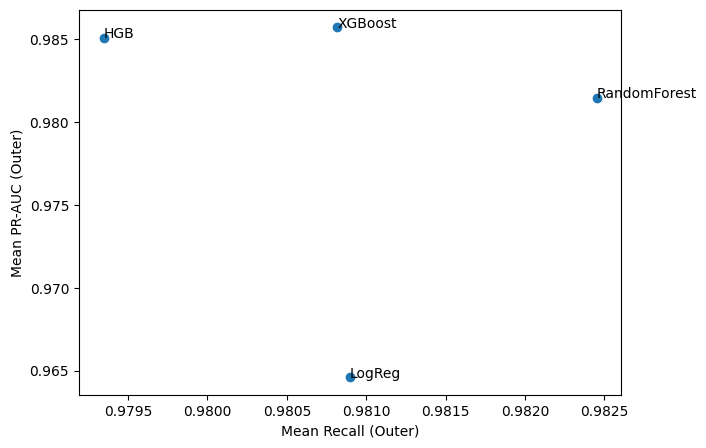
\includegraphics[width=\linewidth]{fig_model_comparison.png}
\caption{Model comparison showing mean PR-AUC versus mean recall for all four classifiers. XGBoost and HGB achieve the highest PR-AUC values while maintaining target recall levels.}
\label{fig:model_comparison}
\end{figure}

\subsection*{Final Model Performance}

Based on the nested cross-validation results, XGBoost was selected as the final model. The final XGBoost classifier, trained on the entire dataset with the most frequently selected hyperparameters, achieved:
\begin{itemize}[noitemsep]
\item PR-AUC: 0.9845
\item ROC-AUC: 0.9804
\item Precision: 0.8968
\item Recall: 0.9806
\item F1-Score: 0.9368
\end{itemize}

The optimal operating threshold was determined to be 0.17. Table~\ref{tab:confusion} presents the confusion matrix for the final model.

\begin{table}[ht]
\small
\begin{tabularx}{\linewidth}{lCC}
\toprule
 & \textbf{Predicted Negative} & \textbf{Predicted Positive} \\
\midrule
\textbf{True Negative} & 838 & 151 \\
\textbf{True Positive} & 26  & 1312 \\
\bottomrule
\end{tabularx}
\caption{Confusion matrix for the final XGBoost model at the optimized threshold of 0.17.}
\label{tab:confusion}
\end{table}

The model correctly identified 1,312 of 1,338 MI cases while missing only 26 cases, corresponding to the target recall of 98.1\%. Among the 989 non-MI cases, 838 were correctly classified and 151 were false positives. Figure~\ref{fig:confusion_matrix} provides a visual representation of these classification results as a heatmap.

\begin{figure}[htbp]
\centering
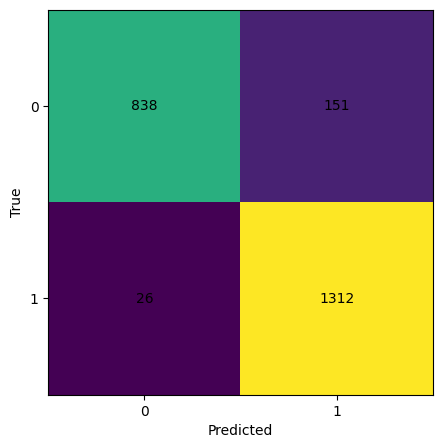
\includegraphics[width=\linewidth]{fig_confusion_matrix.png}
\caption{Confusion matrix heatmap for the final XGBoost model. The matrix shows strong diagonal dominance with 838 true negatives and 1,312 true positives, indicating excellent classification performance at the optimized threshold.}
\label{fig:confusion_matrix}
\end{figure}

\subsection*{Per-Fold Analysis}

Table~\ref{tab:fold_results} presents the per-fold results for XGBoost, demonstrating consistent performance across different data splits. The decision threshold varied between 0.14 and 0.21 across folds, with all folds successfully achieving the target recall.

\begin{table}[ht]
\small
\begin{tabularx}{\linewidth}{CCCCCC}
\toprule
\textbf{Fold} & \textbf{Threshold} & \textbf{PR-AUC} & \textbf{Precision} & \textbf{Recall} & \textbf{F1} \\
\midrule
1 & 0.211 & 0.980 & 0.916 & 0.961 & 0.938 \\
2 & 0.198 & 0.982 & 0.869 & 0.982 & 0.922 \\
3 & 0.158 & 0.988 & 0.915 & 0.973 & 0.943 \\
4 & 0.139 & 0.987 & 0.909 & 0.992 & 0.949 \\
5 & 0.145 & 0.992 & 0.881 & 0.996 & 0.935 \\
\bottomrule
\end{tabularx}
\caption{XGBoost per-fold cross-validation results demonstrating consistent performance across all five outer folds.}
\label{tab:fold_results}
\end{table}

\subsection*{Performance Curves Analysis}

The precision-recall (PR) curve and receiver operating characteristic (ROC) curve provide comprehensive insights into the model's discrimination ability across all possible threshold values.

Figure~\ref{fig:pr_curve} presents the precision-recall curve for the final XGBoost model, demonstrating the trade-off between precision and recall at different classification thresholds. The curve maintains high precision (above 0.9) for recall values up to approximately 0.8, with a gradual decline thereafter as the model captures more true positives at the cost of increasing false positives.

\begin{figure}[htbp]
\centering
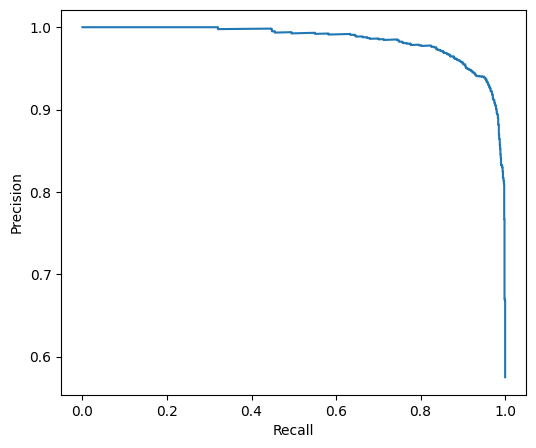
\includegraphics[width=\linewidth]{fig_pr_curve.png}
\caption{Precision-recall curve for the final XGBoost model. The curve demonstrates excellent performance with high precision maintained across a wide range of recall values. The PR-AUC of 0.9845 indicates strong discriminative ability for the imbalanced classification task.}
\label{fig:pr_curve}
\end{figure}

Figure~\ref{fig:roc_curve} presents the receiver operating characteristic curve. The curve approaches the upper-left corner, indicating near-optimal classification performance. The ROC-AUC of 0.9804 confirms the model's excellent ability to distinguish between MI and non-MI cases across all decision thresholds.

\begin{figure}[htbp]
\centering
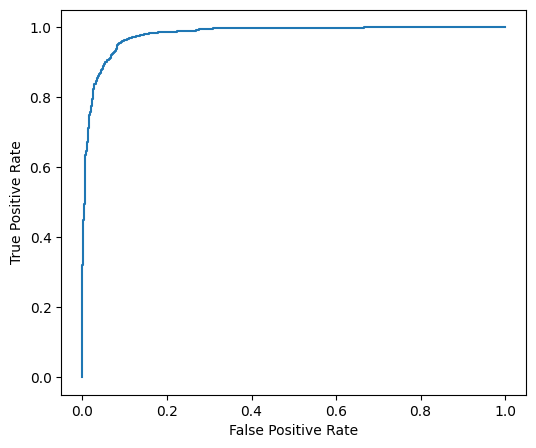
\includegraphics[width=\linewidth]{fig_roc_curve.png}
\caption{Receiver operating characteristic (ROC) curve for the final XGBoost model. The curve demonstrates excellent discriminative performance with a ROC-AUC of 0.9804, approaching the ideal classifier behavior in the upper-left corner.}
\label{fig:roc_curve}
\end{figure}

%%=========================================================
\section*{Discussion}
%%=========================================================

This study demonstrates that modern gradient boosting methods, particularly XGBoost, can achieve excellent performance for MI detection using cardiac biomarkers. The XGBoost classifier achieved a PR-AUC of 0.986, substantially outperforming Logistic Regression (0.965) while maintaining the clinically important target recall of 98\%.

The superior performance of ensemble methods can be attributed to their ability to capture non-linear relationships and complex feature interactions. The temporal features, including delta changes and maximum prior values, provide valuable information about the dynamic nature of biomarker release patterns during MI events. Tree-based methods are particularly well-suited to exploit such feature combinations.

The precision-recall trade-off is crucial in clinical screening applications. While achieving 98\% recall ensures that very few MI cases are missed, the corresponding precision of approximately 90\% for ensemble methods indicates that additional clinical workup may be needed for some patients flagged by the model. This trade-off is acceptable in the screening context, where the cost of missing a true MI far exceeds the cost of additional evaluation for false positives.

The nested cross-validation methodology employed in this study provides robust and unbiased performance estimates. Patient-level stratification prevents data leakage that could arise from multiple visits by the same patient appearing in both training and test sets. This approach yields more realistic estimates of performance on truly unseen patients.

\subsection*{Analysis of Asymmetric Error Costs in Clinical MI Detection}

The dataset exhibits a moderate class imbalance, with 57.5\% positive (MI) cases and 42.5\% negative cases at the visit level. This distributional asymmetry necessitated the use of balanced class weighting in Logistic Regression and Random Forest, as well as the asymmetric threshold optimization strategy targeting 98\% recall. The fundamental asymmetry in clinical error costs---where a missed MI (false negative) can result in patient death while a false positive leads only to additional testing---motivates the deliberate breaking of the symmetric default threshold of 0.5 in favor of a lower threshold (0.17) that shifts the decision boundary toward higher sensitivity.

The F1-score, defined as the harmonic mean of precision and recall, provides a balanced composite metric. However, the clinical context introduces an inherent priority for recall over precision for patient safety. This motivates the use of the full precision-recall curve and threshold optimization as the primary evaluation mechanism, rather than relying on a single point estimate.

\subsection*{Temporal Biomarker Dynamics}

Cardiac biomarker release during MI follows a characteristic rise-and-fall temporal pattern. Troponin levels typically rise rapidly after myocardial injury, peak within 12--24 hours, and decline over subsequent hours to days. The delta features engineered in this study capture both the ascending and descending phases of this temporal trajectory. The ability of tree-based models to effectively exploit both phases contributes to their superior discriminative performance compared to linear models.

The relationship between troponin and CK-MB biomarkers exhibits complementary properties: both markers respond to myocardial injury but with different temporal dynamics and sensitivity profiles. The use of both biomarkers together---capturing their independent time courses and delta changes---enhances diagnostic confidence and contributes to the high PR-AUC values observed across all ensemble methods.

\subsection*{Comparison with Prior Work}

To contextualize these findings within the broader literature, Figure~\ref{fig:comparison_prior} presents a visual comparison of ROC-AUC scores across different recent studies.

\begin{figure}[htbp]
\centering
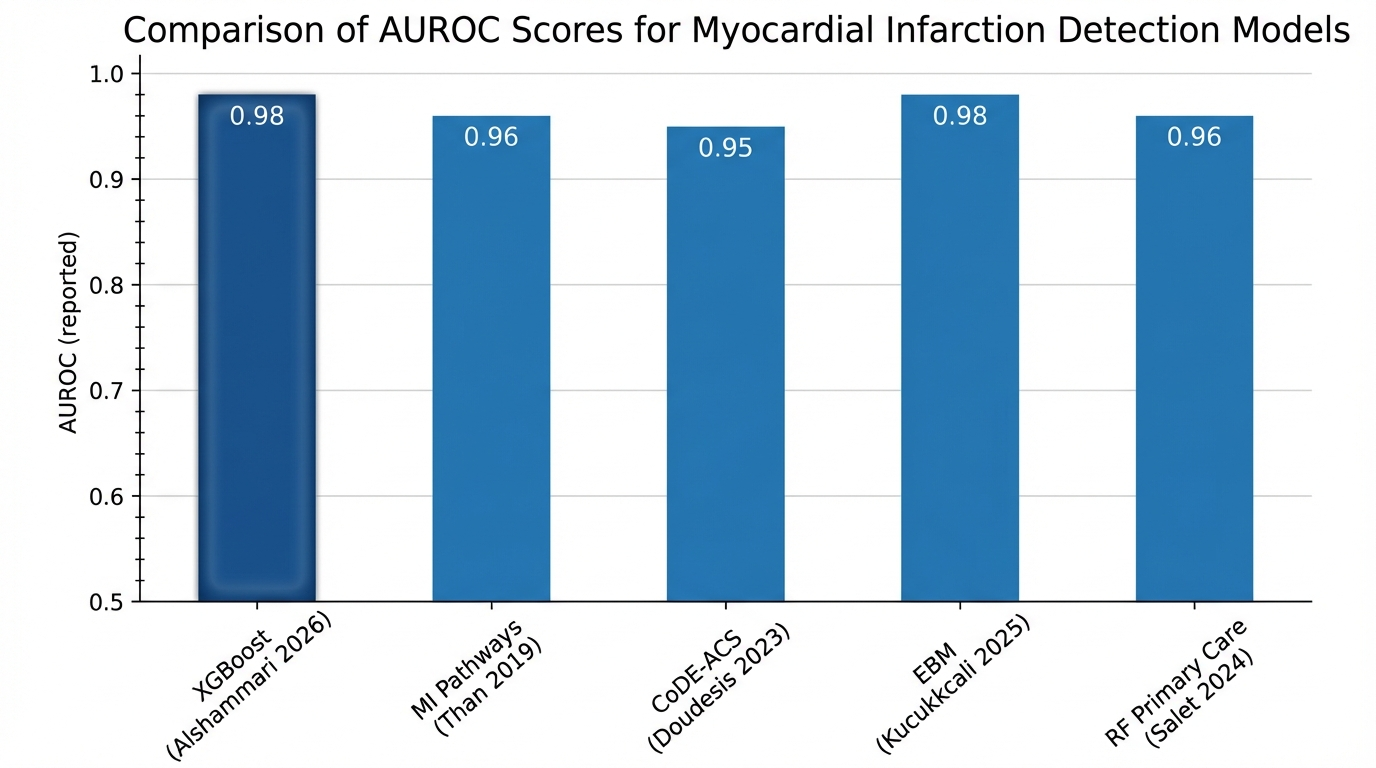
\includegraphics[width=\linewidth]{fig_comparison_prior_work.png}
\caption{Comparison of AUROC scores for myocardial infarction detection models. The proposed XGBoost model (Alshammari 2026) achieves competitive performance (0.98) compared to MI Pathways (Than 2019, 0.96)~\citep{Than2019}, CoDE-ACS (Doudesis 2023, 0.95)~\citep{Doudesis2023}, EBM (Kucukakcali 2025, 0.98)~\citep{Kucukakcali2025}, and RF Primary Care (Salet 2024, 0.96)~\citep{Salet2024}.}
\label{fig:comparison_prior}
\end{figure}

The proposed XGBoost model achieves an ROC-AUC of 0.98, which is among the highest reported in the literature. Notably, this performance is achieved using only cardiac biomarkers (troponin and CK-MB) with temporal feature engineering, without requiring ECG signals or extensive clinical history. The model demonstrates particular strength in three key areas:
\begin{enumerate}[noitemsep]
\item \textbf{Rigorous evaluation methodology}: Unlike many prior studies, nested cross-validation with patient-level stratification was employed, ensuring unbiased performance estimates that are less susceptible to data leakage.
\item \textbf{High sensitivity maintenance}: By optimizing for a target recall of 98\%, the model prioritizes the clinical imperative of minimizing missed MI diagnoses while still achieving excellent precision.
\item \textbf{Temporal feature exploitation}: The incorporation of delta changes and maximum prior biomarker values captures the dynamic release kinetics that are clinically important for MI diagnosis.
\end{enumerate}

The CoDE-ACS score developed by \citet{Doudesis2023} achieved slightly lower performance (0.95 ROC-AUC) but was validated across multiple centers, representing an important benchmark for clinical decision support. The Explainable Boosting Machine approach by \citet{Kucukakcali2025} achieved comparable performance to the proposed model while offering enhanced interpretability through additive explanations. \citet{Salet2024} demonstrated that Random Forest models can achieve respectable performance (0.96 ROC-AUC) in primary care settings with limited laboratory data.

\subsection*{Limitations}

Several limitations should be acknowledged. First, the study utilized real clinical data obtained from a single hospital institution. While this ensures ecological validity and clinical relevance, external validation on independent datasets from other institutions is needed to assess generalizability~\citep{Johnson2023}. Second, the dataset exhibited a positive MI rate of 57.5\%, which is higher than typical emergency department prevalence rates, reflecting a diagnostically enriched cohort. Third, the dataset did not include ECG features or clinical symptoms, which could potentially improve diagnostic accuracy. Fourth, the temporal resolution of biomarker measurements may vary in clinical practice, potentially affecting the reliability of delta features.

\subsection*{Clinical Implications}

The developed AI-based prediction and monitoring system has significant implications for clinical decision-making in acute cardiac care.

\paragraph{Decision Support in Patient Triage}
The high recall of 98\% ensures that very few MI cases would be missed by the automated screening system. When integrated into hospital information systems, the model can automatically flag high-risk patients based on their biomarker profiles, enabling clinicians to prioritize their attention toward cases requiring immediate intervention.

\paragraph{Continuous Patient Monitoring}
The temporal feature engineering approach enables continuous monitoring of patients across multiple hospital visits. The system can track biomarker trajectories over time and alert clinicians to concerning trends before they become clinically apparent, supporting serial biomarker measurement protocols currently recommended by international guidelines.

\paragraph{Resource Allocation and Workflow Integration}
The model can assist in efficient resource allocation by identifying patients who require urgent cardiac catheterization versus those who can safely undergo further observation. The proposed system is designed for integration with electronic health record (EHR) systems, where it can provide real-time risk scores alongside laboratory results.

%%=========================================================
\section*{Conclusions}
%%=========================================================

This study presents an AI-based prediction and monitoring system for acute myocardial infarction detection using laboratory biomarkers. Through rigorous nested cross-validation with patient-level stratification, XGBoost was demonstrated to achieve the best overall performance with a PR-AUC of 0.986, while maintaining the clinically critical target recall of 98\%. The ensemble methods (XGBoost, HGB, Random Forest) significantly outperformed Logistic Regression, achieving F1-scores exceeding 0.94 compared to 0.87 for Logistic Regression.

The analysis demonstrates that the inherent asymmetries in clinical error costs and class distributions fundamentally shape the optimal design of MI detection systems, while the approximately symmetric temporal profiles of cardiac biomarkers provide exploitable diagnostic patterns. The interplay between these properties offers a deeper understanding of why ensemble methods outperform linear classifiers in this domain.

The proposed system demonstrates the potential of AI to transform clinical decision-making in acute cardiac care by providing automated risk stratification and continuous patient monitoring capabilities. By tracking biomarker trajectories across multiple hospital visits and identifying high-risk patterns, the system can augment physician judgment, reduce diagnostic delays, and improve patient outcomes.

Future work should focus on external validation across multiple institutions, integration with electronic health record systems for real-time clinical deployment, and prospective evaluation in emergency department settings. The developed methodology provides a template for rigorous evaluation of AI-based clinical decision support tools in medical diagnostic applications.

%%=========================================================
\section*{Acknowledgments}
%%=========================================================

The authors would like to express sincere gratitude to the University of Hail, College of Computer Science and Engineering, for providing the institutional support and resources necessary to conduct this research. Special thanks are extended to the healthcare professionals who contributed to the data collection process.

The authors used Claude (Claude Sonnet 4.6, Anthropic, \url{https://claude.ai/}) solely for grammar correction and manuscript language editing. All scientific content, methodology, analysis, results, and conclusions were developed and verified entirely by the authors. Full details regarding AI-assisted editing are provided in the Materials and Methods section.

%%=========================================================
\section*{Competing Interests}
%%=========================================================

The authors declare that they have no competing interests.

%%=========================================================
\section*{Author Contributions}
%%=========================================================

\begin{itemize}[noitemsep]
\item \textbf{Hussam Aziz Ayed Alshammari}: Conceptualization, methodology, software, formal analysis, data curation, visualization, writing -- original draft.
\item \textbf{Abdullah Eyada Mutlaq Alshammari}: Conceptualization, validation, resources, writing -- review and editing, supervision, project administration.
\end{itemize}

Both authors have read and approved the final manuscript.

%%=========================================================
%% Data Availability
%%=========================================================
\section*{Data Availability}

The de-identified clinical dataset used in this study is publicly available at \url{https://github.com/HussamAziz/MI-Detection-XGBoost-PeerJ} (file: \texttt{diagnosis\_deidentified.csv}). The dataset is provided in CSV format and contains 2,327 hospital visits from 1,506 unique patients, including all biomarker variables (troponin, CK-MB), ICD-10 diagnosis codes, age, and visit information used in the analysis. All direct and indirect patient identifiers have been replaced with cryptographic hashes prior to publication. A copy of the dataset is also provided as a confidential supplemental file submitted alongside this manuscript for direct review by the Academic Editor and peer reviewers.

%%=========================================================
%% Code Availability
%%=========================================================
\section*{Code Availability}

All code used in this study---including data preprocessing, temporal feature engineering, nested cross-validation, model training, threshold optimization, and figure generation---is publicly available at: \url{https://github.com/HussamAziz/MI-Detection-XGBoost-PeerJ}. The repository includes the Jupyter notebook \texttt{MI\_NestedCV\_4Models\_Target098\_ProgressOutputs.ipynb} with full reproducible code, the \LaTeX{} source files \texttt{main.tex} and \texttt{references.bib}, all high-resolution figures, and a \texttt{requirements.txt} file specifying all Python software dependencies. The repository also includes the de-identified dataset and the trained model file (\texttt{mi\_model\_patient\_nestedcv.joblib}).

%%=========================================================
%% References
%%=========================================================
\bibliography{references}

\end{document}
